% nim 012 dag
\documentclass[12pt]{article}
\usepackage{calc}
\usepackage{tikz}
\usetikzlibrary{arrows,decorations.markings}
\tikzstyle{vertex}=[rectangle, draw, inner sep=5pt, minimum size=18pt]
\newcommand{\vertex}{\node[vertex]}
\newcounter{Angle}

\pagestyle{empty}
\begin{document}
{%\large\bf
\[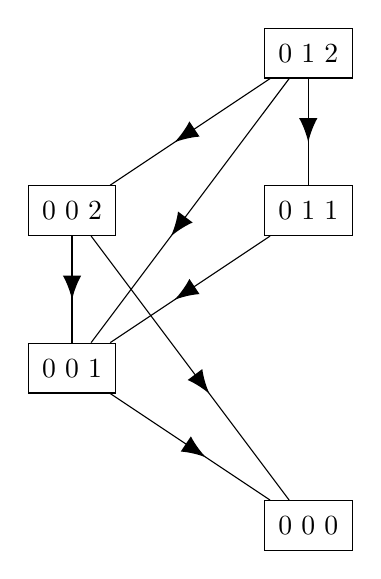
\begin{tikzpicture}[x=1.5cm, y=2cm
    ,every edge/.style={
        draw,
        postaction={decorate,
                    decoration={markings,mark=at position .6 with
		    {\arrow[line width=2pt,black]{latex}}} } }
]
\vertex (012) at (2, 3) {0 1 2};
\vertex (002) at (0, 2) {0 0 2};
\vertex (011) at (2, 2) {0 1 1};
\vertex (001) at (0, 1) {0 0 1};
\vertex (000) at (2, 0) {0 0 0};
\path
(012) edge (002) edge (001) edge (011)
(002) edge (001) edge (000)
(011) edge (001) 
(001) edge (000) 
;
\end{tikzpicture}\]
\end{document}
